% !TeX spellcheck = en_GB
\begin{figure}[!htb]
  \setlength{\unitlength}{\textwidth}

        \begin{picture}(1,0.4)(-0.02,0)

 
      
      \put(0.08,0.02){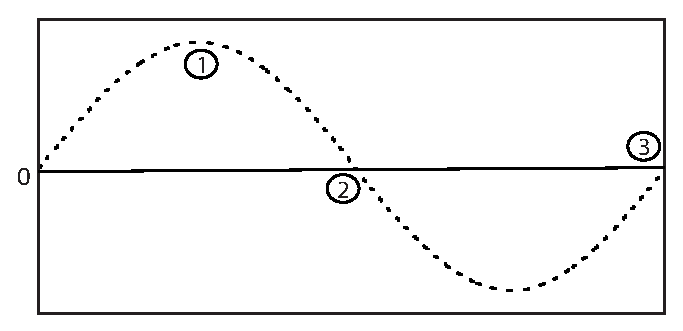
\includegraphics[width=0.75\unitlength]{./chapter-cross-sections/fnp/fsi_flow_sketch.eps}}

      %\put(0.46,0.00){\massdamp}
      
      
     
       %\put(0.03,0.235){$\displaystyle\frac{P_{m}}{\rho \mathcal{A}U^3 }$}
      

      %\put(0.095,0.218){\small(a)}
      %\put(0.565,0.218){\small(b)}
      
    \end{picture}

  \caption{Illustration of the time history of velocity depicting the points considered to obtained time averaged flow-field data. The points considered are: the point where the velocity is at its maximum; where the velocity is zero and continues to decrease; where the velocity is zero and continues to increase.}
    \label{fig:FSI_sketch}
\end{figure}

 %vspace{10cm}
